\documentclass{article}
\usepackage[margin=1in]{geometry}
\usepackage{amsmath}
\usepackage{graphicx}




\begin{document}

\title{\textbf{Airfoil Selection - Iteration 2}}
\author{Abigail Gries}
\maketitle

As the OpenUAS team begins the second design of the UAS, one design choice that can potentially be improved upon is the airfoil. This document outlines the process and resources that the OpenUAS team used to reevaulate the original airfoil and compare it to other options. 

\section*{Step 1 - New Airfoil Candidates}

The team's UAS will be flying at low velocities and low Reynold's numbers due to budget, legal, and technological constraints. Originally, research was first done to find potential airfoils that perform well at these conditions. Various resources were used to locate qualified airfoils, however, one academic paper proved to be very useful [1]. From this paper, three airfoils were selected: NACA 0015, NACA 0019, and NACA 4512. These specific airfoils were chosen because they had dominant airspeeds in the same range of our UAS (15 m/s to 30 m/s) and they performed well in the optimization process detailed in the paper [1]. During the first airfoil selection iteration, the NACA 0015 and NACA 0019 airfoils were eliminated. As such, these two airfoil will not be evaluated again. Instead, three other new airfoils, Clark Y (11.7\% smoothed), S1223, and AG35 were chosen. The Clark Y and S1223 airfoils were suggested by Catherine Sener, while the AG35 was suggested by Logan Gross. All three of these airfoils will be analyzed and compared to the current airfoil, NACA 4512. 

\section*{Step 2 - XFLR5 Analysis}

XFLR5 was used once again as the main analysis tool. The Reynolds number selected for the analysis was 172,000. This corresponds to a speed of 20 m/s (~44.7 mph), chord width of 0.122 m (0.4 ft), and kinematic viscosity of $1.4207\times10^{-5}$ m\^2/s. The corresponding mach number is 0.059. Once again, a Type 1 analysis was performed with a Ncrit value of 9. Data was generated for angles of attack ranging from -5 degrees to 15 degrees. Once the program completed the analysis for all of the airfoils, the polars were exported to csv files to be further analyzed, as detailed below. 

\section*{Step 3 - Calculations}

Using the csv files created by XFLR5, two different plots were created for each airfoil. The coefficient of lift and the angle of attack were plotted against each other. From this graph, important characteristics of the airfoil could be determined. Specifically, the coefficient of zero lift drag, the maximum coefficient of lift, and the stall angle of attack were all estimated using the plots. The coefficient of zero lift drag, or $Cl_{0}$, was determined by finding the y-intercept of the  $Cl$ vs $\alpha$ plot. The maximum coefficient of lift, $Cl_{max}$, is the highest coefficient of lift in the given range of alpha, so the maximum peak of the curve was selected for each airfoil. The stall angle of attack, $\alpha_{stall}$, was estimated as the angle in degrees associated with the end of the linear range of each plot. Another plot was also created using the data from the csv files. The coefficient of lift vs coefficient of drag, or $Cl$ vs $Cd$, plot was produced, and from this plot, the minimum coefficient of drag and the maximum of efficiency of the airfoils were estimated. The minimum coefficient of drag, $Cd_{min}$, is the x-intercept of the $Cl$ vs $Cd$ plot. The maximum aerodynamic efficiency, or $E_{max}$, is the point with the highest slope on the plot. These characteristics of each airfoil, the coefficient of zero lift drag, the maximum coefficient of lift, the stall angle of attack, the minimum coefficient of drag, and the maximum aerodynamic efficiency, are all key parameters that were used in selecting the most appropriate airfoil for the OpenUAS project. The values for each parameter are shown in the table below.\\\\

\begin{figure}[!h]
\begin{center}
	\includegraphics[scale=0.7]{NACA4512clvsalpha_new.png}
	\caption{NACA 4512 $Cl$ vs $\alpha$}
	\label{Figure 1:}
\end{center}
\end{figure}

\begin{figure}[!h]
\begin{center}
	\includegraphics[scale=0.7]{NACA4512clvscd_new.png}
	\caption{NACA 4512 $Cl$ vs $Cd$}
	\label{Figure 2:}
\end{center}
\end{figure}
\newpage

\begin{figure}[!h]
\begin{center}
	\includegraphics[scale=1]{Clarkyclvsalpha.png}
	\caption{Clark Y $Cl$ vs $\alpha$}
	\label{Figure 3:}
\end{center}
\end{figure}

\begin{figure}[!h]
\begin{center}
	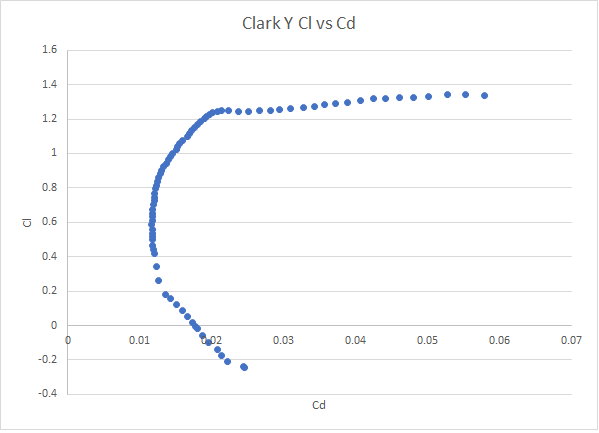
\includegraphics[scale=1.1]{clarkyclvscd.png}
	\caption{Clark Y $Cl$ vs $Cd$}
	\label{Figure 4:}
\end{center}
\end{figure}

\newpage
\begin{figure}[!h]
\begin{center}
	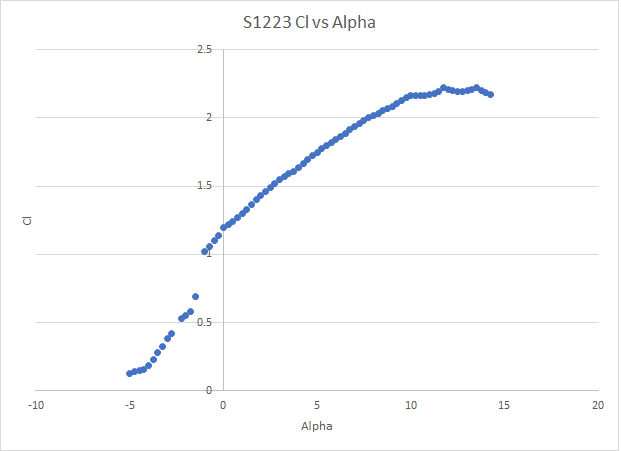
\includegraphics[scale=1]{s1223clvsalpha.png}
	\caption{S1223 $Cl$ vs $\alpha$}
	\label{Figure 5:}
\end{center}
\end{figure}

\begin{figure}[!h]
\begin{center}
	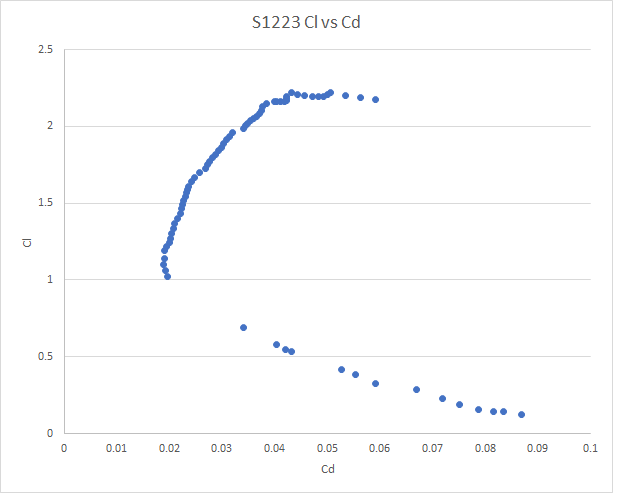
\includegraphics[scale=1]{s1223clvscd.png}
	\caption{S1223 $Cl$ vs $Cd$}
	\label{Figure 6:}
\end{center}
\end{figure}

\newpage
\begin{figure}[!h]
\begin{center}
	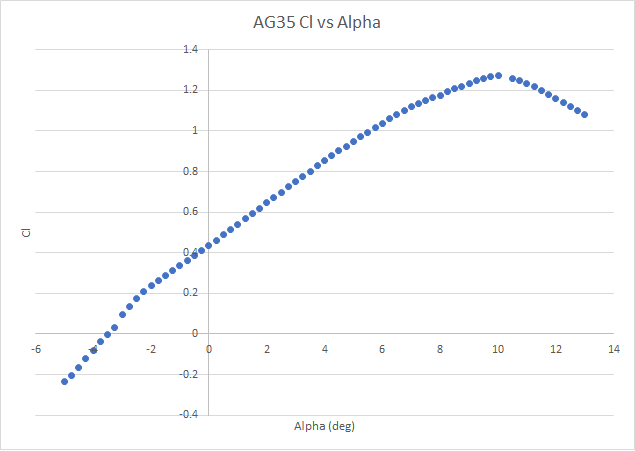
\includegraphics[scale=1]{ag35clvsalpha.png}
	\caption{AG35 $Cl$ vs $\alpha$}
	\label{Figure 7:}
\end{center}
\end{figure}

\begin{figure}[!h]
\begin{center}
	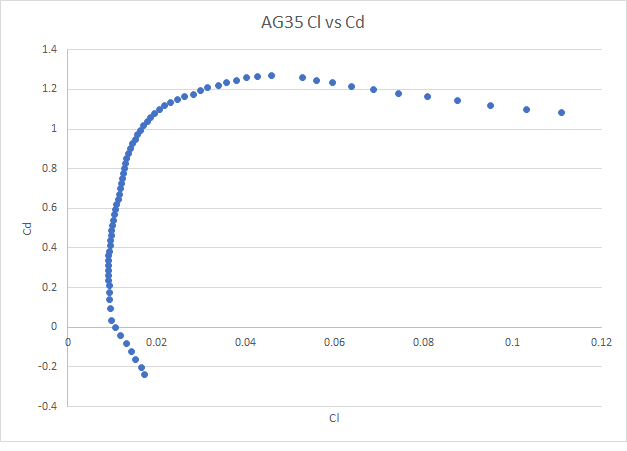
\includegraphics[scale=1]{ag35clvscd.png}
	\caption{AG35 $Cl$ vs $Cd$}
	\label{Figure 8:}
\end{center}
\end{figure}

\newpage

\section*{Results}
\begin{tabular}[pos]{| c | c | c | c | c |}
\hline
Parameter & NACA 4512 & S1223 & Clark Y & AG35 \\ \hline
$Cl_{0}$ & 0.4742 & 1.1949 & 0.499 & 0.4356   \\ \hline
$Cl_{max}$  & 1.285 & 2.1646 & 1.2475 & 1.2716 \\ \hline
$\alpha_{stall}$ & 7.25 & 9.75 & 8.5 & 7.75 \\ \hline
$Cd_{min}$ & 0.01958 & $>$0.09 & 0.0177 & 0.01066 \\ \hline
$E_{max}$ & 78.95 & 68.03 & 69.495 & 64.595 \\ \hline
\end{tabular}

\section*{Step 4 - Weighted Scoring Method}\section*{Step 4 - Weighted Scoring Method}

In order to select the most appropriate airfoil based on the parameters outlined in the Calculations section, a weighted scoring method was used. This method is a modified version of the process used in reference [2]. A ranking place, 1st, 2nd, or 3rd, is given to each airfoil for each parameter. Each place has the following points associated with it: 4 points for 1st place, 3 points for 2nd place, 2 points for 3rd place, and 1 point for 4th place. Then, each parameter has a weight associated with it. The points an airfoil receives for each parameter are multiplied by the weight or "multiplier." Finally, all the weighted points are added up. The table below shows the ranking, multiplier, and total points for each airfoil. \\ \\

\begin{tabular}[pos]{| c | c | c | c | c | c | c |}
\hline
Parameter & Evaluation & NACA 4512 & S1223 & Clark Y & AG35 & Multiplier \\ \hline
$Cl_{0}$ & Closest to cruise is best & 3rd & 1st & 2nd & 4th & 1.2  \\ \hline
$Cl_{max}$ & Highest is best & 2nd & 1st & 4th & 3rd & 1.25 \\ \hline
$\alpha_{stall}$ & Highest is best & 4th & 1st & 2nd & 3rd & 1.15 \\ \hline
$Cd_{min}$ & Lowest is best & 3rd & 4th & 2nd & 1st & 1.15 \\ \hline
$E_{max}$ & Highest is best & 1st & 3rd & 2nd & 4th & 1.25  \\ \hline
Total Points & & \textbf{14.6} & \textbf{18.05} & \textbf{15.5} & \textbf{11.85} & \\ \hline
\end{tabular}


\section*{Step 5 - Selection}
Although the airfoil with the highest score was S1223, the OpenUAS team did not decide to go with this airfoil. The team instead chose Clark Y. The reason for this decision was due to the shape of the S1223 airfoil. This airfoil is highly cambered, making it difficult to manufacture. Additionally, this type of airfoil is typically used for a glider. The team chose Clark Y because it had the second best score and improved upon the NACA 4512 selection. This airfoil is commonly used in UAS design as well. 

\section*{References}

[1] V. Brusov \& V. Petruchik. (2011). Design Approach for Selection of Wing Airfoil with Regard to Micro-UAVs. International Micro Air Vehicle Conference, Netherlands, September 2011. Delft University of Technology. Retreived from: https://repository.tudelft.nl/islandora/object/uuid:2b261a19-fae4-44dd-ac04-1113ebc7c89b?collection=research \\

\noindent [2] Ngo, Khanh \& Thien Loc, Huynh. (2016). Airfoil Selection for Fixed Wing of Small Unmanned Aerial Vehicles. 881-890. 10.1007/978-3-319-27247-4\_73.


\end{document}
